%%%%%%%%%%%%%%%%%%%%%%%%%%%%%%%% 
\section{The 35-ton Prototype} 
\label{sec:proto-35t}

When first conceived, the 35t prototype cyrostat was constructed to demonstrate that a non-evacuable membrane cryostat can satisfy the less-than-200-parts-per-trillion (ppt) requirement on oxygen contamination of the liquid argon in the detector and maintain that level stably.
%
It was intended to prototype a wide variety of issues that construction and 
operation of the far detector would need to address, including procurement of 
materials and services, safety and the processes involved with ensuring the 
cryostat can maintain high-purity liquid argon. 
%
Later it was decided to extend its scope, and to install and operate a small-scale LArTPC and photon detector in the cryostat; this phase will focus on the performance of active detector elements placed directly in the volume of liquid argon.

The membrane cryostat demonstration, completed in 2014, is referred to as ``Phase 1'' and the operation of the TPC is called ``Phase 2.''
Phase 2 is currently under construction and it is planned to take data in summer 2015.

\subsection{Phase 1 - Cryostat Construction and Performance}

The construction of the 35t cryostat addressed a number of issues.
First were project-related issues, such as gaining detailed construction experience, 
developing the procurement and contracting model, and incorporating the design and approval mechanism 
in the Fermilab ES\&H manual, which was necessary because membrane cryostats are designed in accordance
with European and Japanese standards.
Secondly, it addressed technical issues such as %demonstrating 
high-purity operation in this type of 
cryostat and the suitability of the planned LAr-FD construction techniques and materials.

The LBNE project contracted with the Japanese company IHI to build the 35t cryostat at Fermilab.  
It was built in Fermilab's PC-4 facility where the Liquid Argon Purity Demonstrator (LAPD)
\cite{bib:lapdP07005}
is also located, which
allowed for re-use of a large portion of the cryogenic-process equipment installed for LAPD.
The proximity and size (30 tons) of LAPD also offers the possibility using LAPD as 
a partial storage vessel for LAr if the 35t ever needs to be emptied. 
The 35t employs a submersible %LAr 
pump to pump the LAr from the cryostat to the filters. Two pumps were installed for redundancy, but 
only one is used at a time.
Figure~\ref{fig:35cutaway} shows a cutaway view of the cryostat and a photograph of the interior
of the completed cryostat. 

\begin{cdrfigure}[Cutaway view]{35cutaway}{(left) Cutaway view of the 35t cyrostat. (right) Interior
photograph of the completed cryostat.}
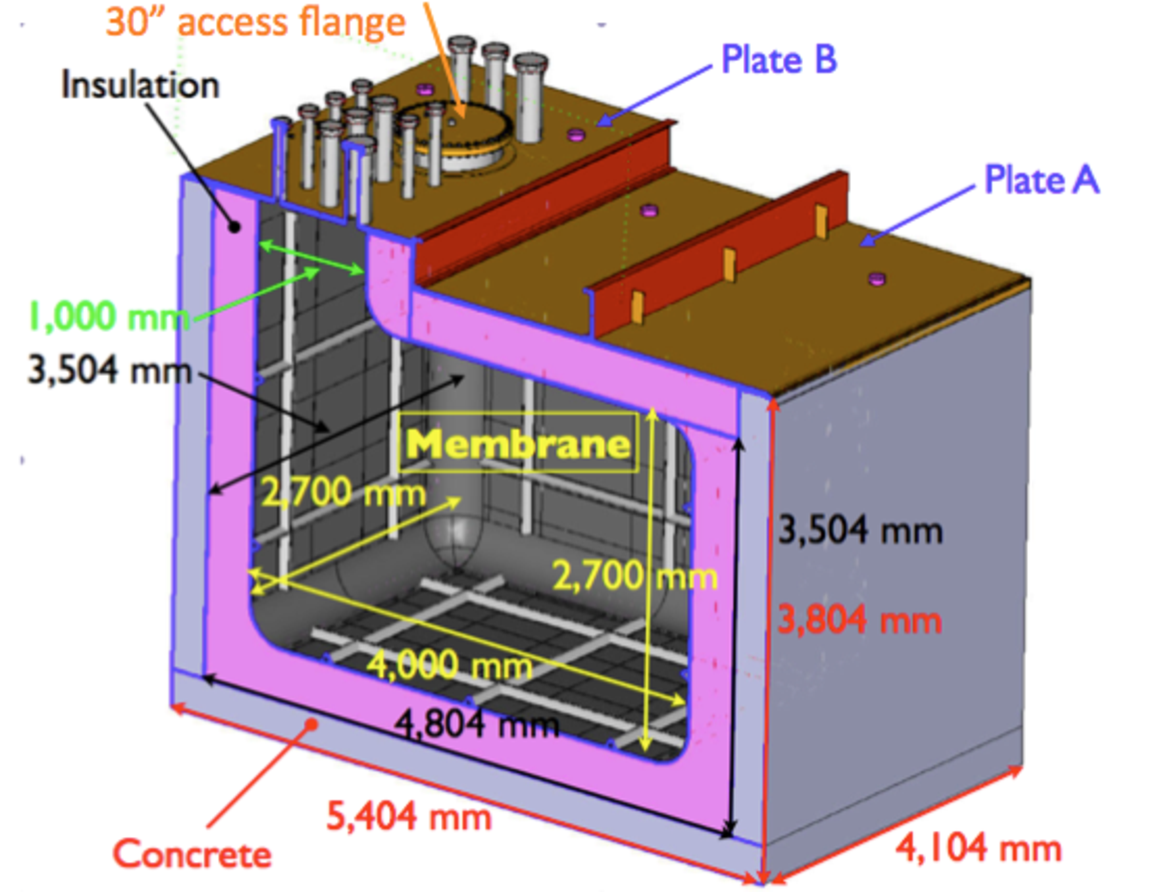
\includegraphics[width=0.60\textwidth]{35TCutaway}
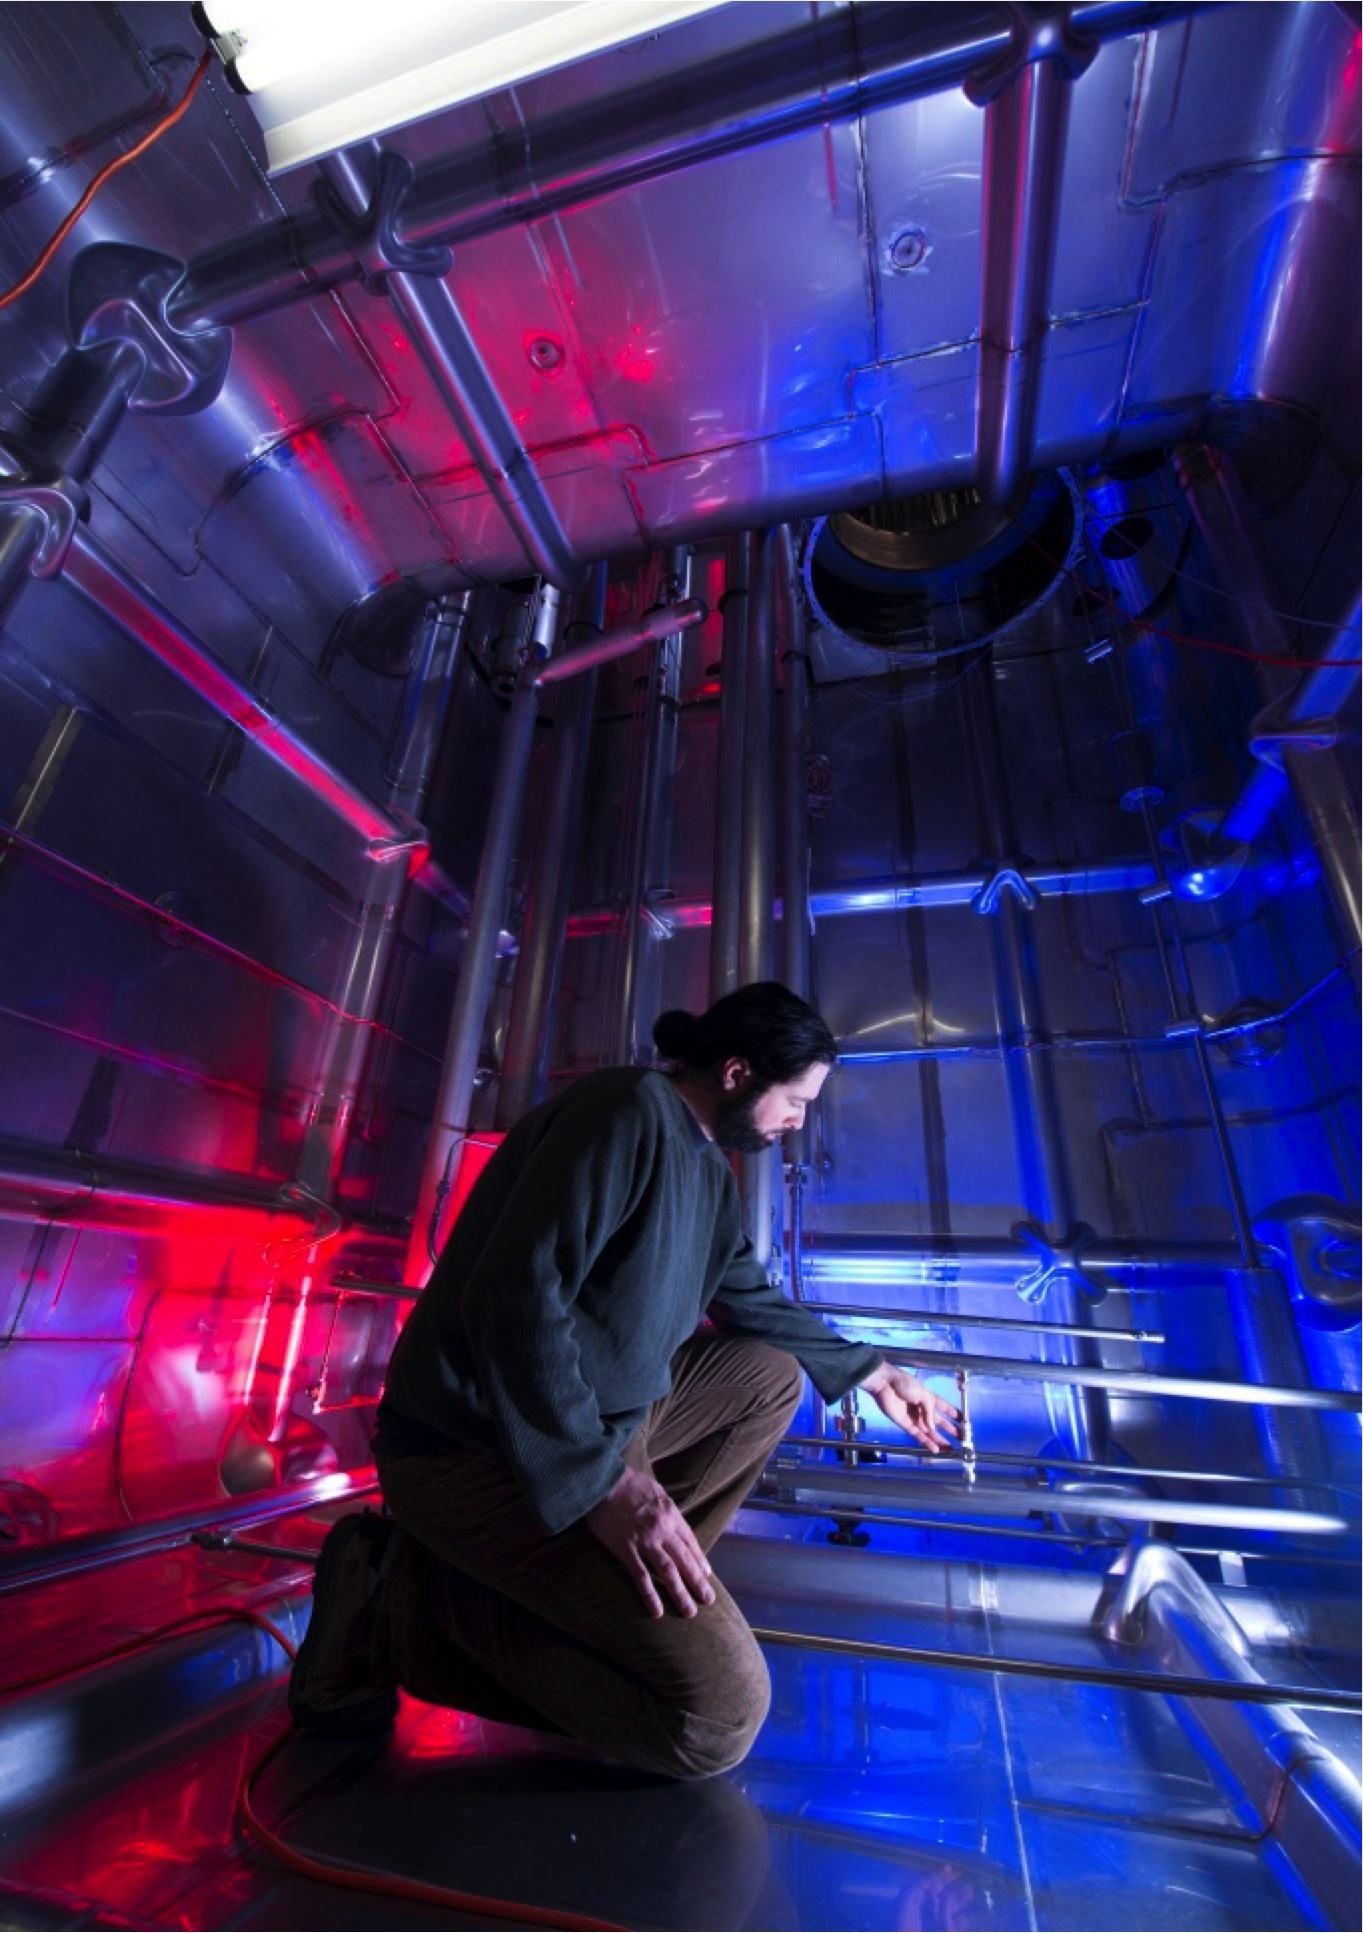
\includegraphics[width=0.35\textwidth]{35TCryo}
\end{cdrfigure}

Table~\ref{tab:35Tdimensions} gives the details of the construction materials and the
dimensions for the 35t.
More information can be found in
\cite{bib:membcryo1573}.
The insulation thickness is 0.4~m rather than the 1.0~m chosen for the reference design.  
The techniques of membrane-cryostat construction were demonstrated to be a fit 
for high-purity TPC service.
Welding of corrugated panels, removal of leak-checking dye penetrant or ammonia-activated
leak-detecting paints, and post-construction-cleaning methods were tested for suitability of service.  

\begin{cdrtable}[35t Details and Dimensions]{ll}{35Tdimensions}
{35t Details and Dimensions}
Parameter & Value \\ \toprowrule
Cryostat Volume	&      29.16 m3\\ \colhline
Liquid Argon total mass	 &     38.6 metric tons\\ \colhline
Inner dimensions	&      4.0 m (L) x 2.7 m (W) x 2.7 m (H)\\ \colhline
Outer dimensions        &      5.4 m (L) x 4.1 m (W) x 4.1 m (H)\\ \colhline
Membrane		&      2.0 mm thick corrugated 304 SS\\ \colhline
Insulation		&      0.4 m polyurethane foam\\ \colhline
Secondary barrier system	   &   0.1 mm thick fiberglass\\ \colhline
Vapor barrier	Normal	  &    1.2 mm thick carbon steel\\ \colhline
Steel reinforced concrete	    &  0.3 m thick layer\\ 
\end{cdrtable}

Once construction was completed, the Argon filling of the cryostat commenced. 
In the first stage, gaseous Ar was used to purge the cryostat and begin the removal
of impurities.
Figure~\ref{fig:35TPurge} graphically shows step 1 of the purification process, removal of the ambient air. The initial state, $t=0$, reflects the initial values for oxygen, water and nitrogen in the ``dry air'' state. This is followed by the Piston Purge.
These measurements are made by a variety of %gas 
monitors that sample the gas in the cryostat. 

\begin{cdrfigure}[Gas Ar Purge and Recirculation]{35TPurge}{Gas phase of removing impurities in the 35t. These quantities are being measured by various gas analyzers. The first stage of the purification is a process called the ``Piston Purge''.  The second stage is ``Recirculation with Filtering''. The gap between the two steps was due to troubleshooting a leak.}
  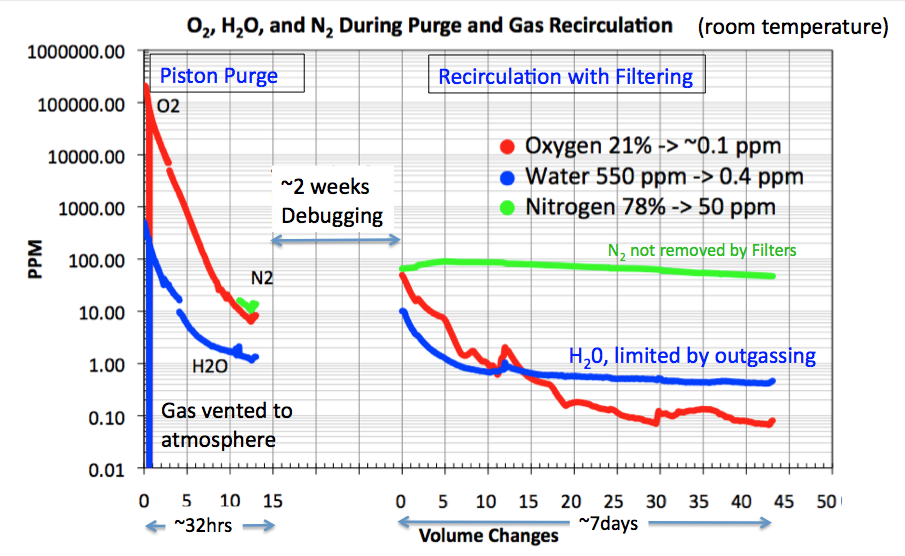
\includegraphics[width=0.8\textwidth]{35TPurgeAndRecirc}
\end{cdrfigure}

Figure~\ref{fig:35TElectronLifetime} shows the electron lifetime from the start of the LAr Pump operation until the end of the Phase 1 run. In general, the electron lifetime improved as a function of pump 
on-time, but there were several incidents that spoiled the lifetime. \fixme{revisit this sentence} These will be discussed in the next section.

\begin{cdrfigure}[35t Electron Lifetime]{35TElectronLifetime}{LAr electron lifetmes as measured by 
Cryostat Purity Monitors. Significant events are annotated on the plot. Major divisions on horizontal axis 
are one week periods. Equivalent purity levels are shown as dashed horizontal lines.}
  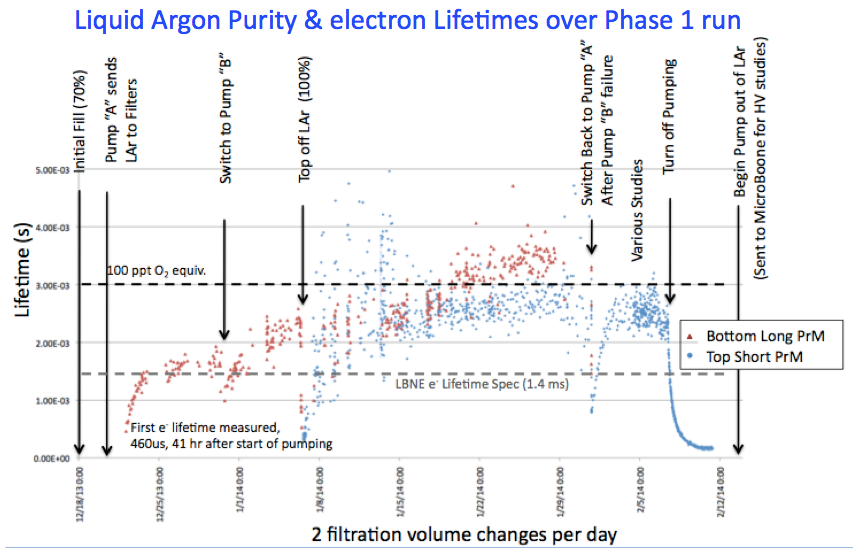
\includegraphics[width=0.7\textwidth]{35TElectronLifetime.png}
\end{cdrfigure}

\subsection{Phase 2 - Installation of Active Detectors}
Phase 2 of the the 35t prototype involves installing a fully operational TPC and photon detector into 
the previously built cryostat.
The prototype will be filled with liquid argon and operated for a several-month-long cosmic ray run. 
External plastic scintillator paddles placed around the cryostat will be used to produce
trigger signals as well as rough position measurements of the incoming cosmic rays.
Installation of the TPC into the cryostat is expected in April 2015 and 
commissioning is expected to begin in June 2015.
%Figure~\ref{fig:tpc-35ton-trial} shows the trial assembly of the TPC outside of the cryostat. 
Figure~\ref{fig:35TTPC} shows a model of the TPC inside the cryostat and a trial assembly of
the TPC done outside of the cyrostat. 

\subsection{35t Phase 2 TPC Design}

\begin{cdrfigure}[35t with TPC]{35TTPC}{(left) 35t Cryostat with TPC and photon detectors installed. 
Note separate drift regions on ``near'' and ``far'' sides.
The near side drift length is close to what is proposed for the far detector. The far
side has a shorter drift length due to lack of space.
(right) A trial assembly of the TPC.
}
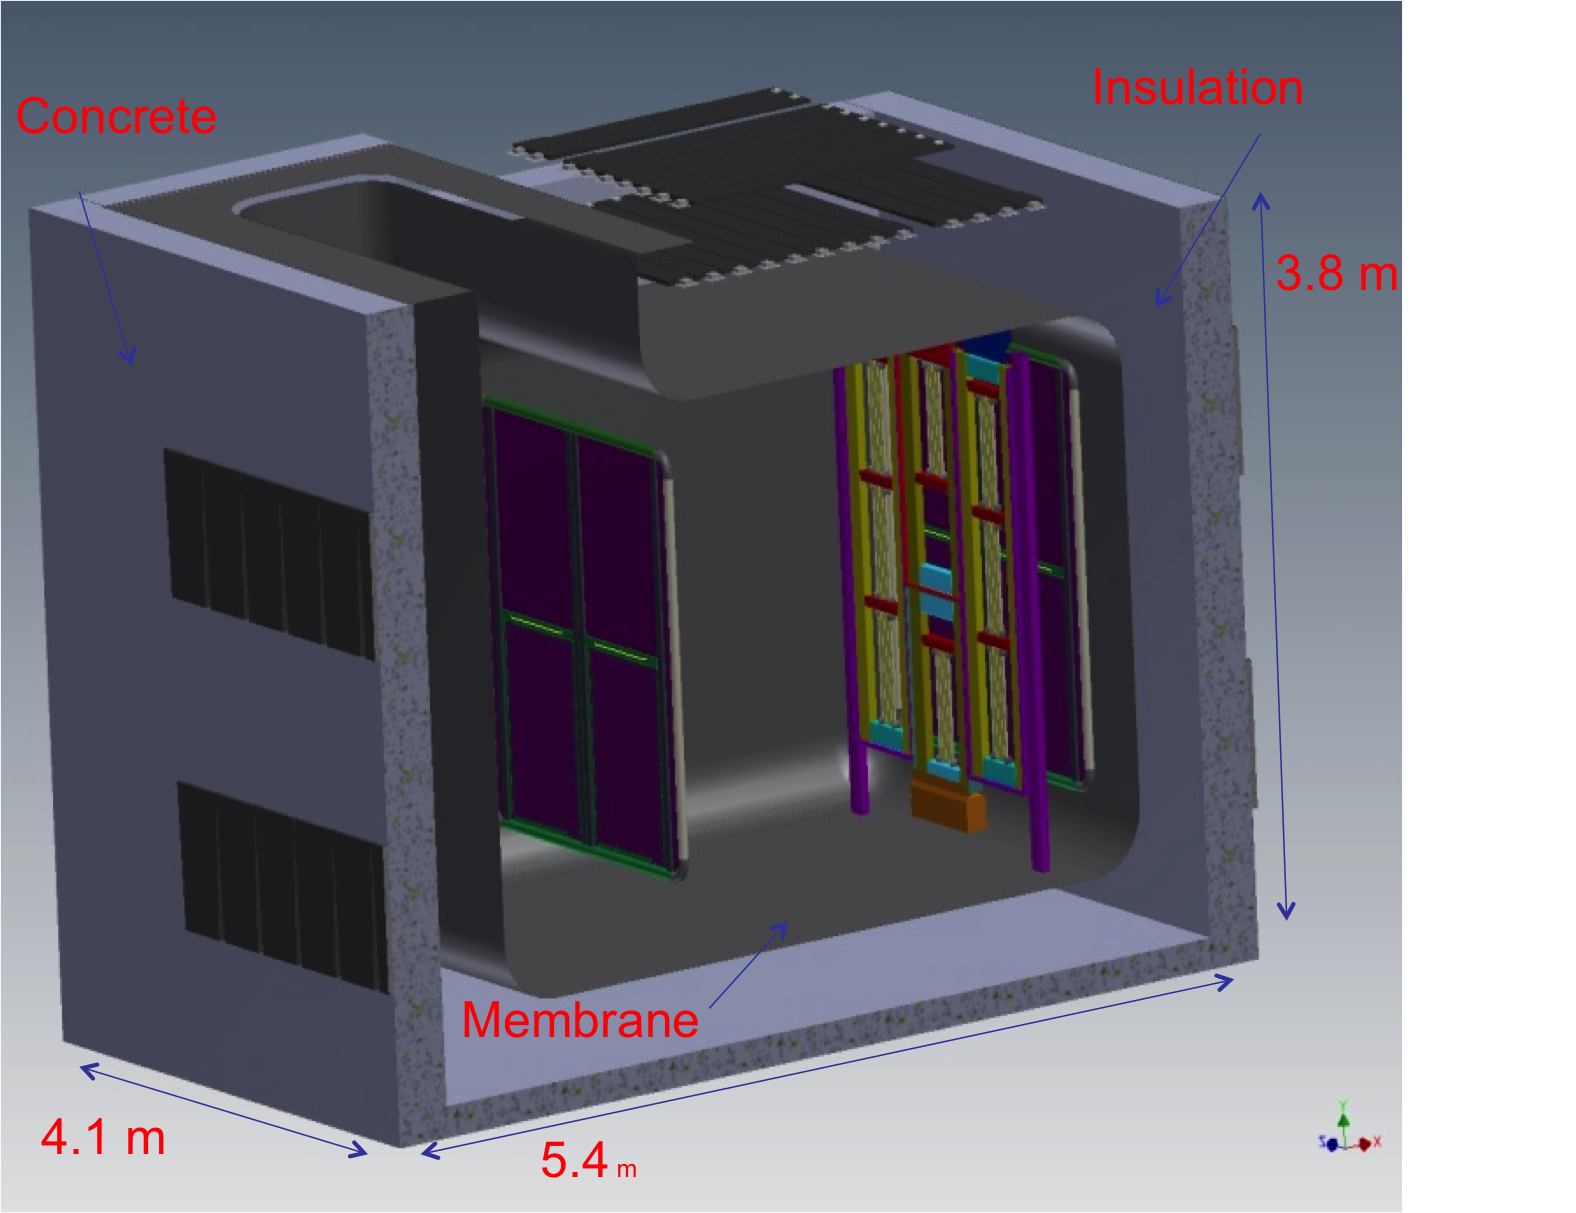
\includegraphics[width=0.55\textwidth]{35TTPC}  
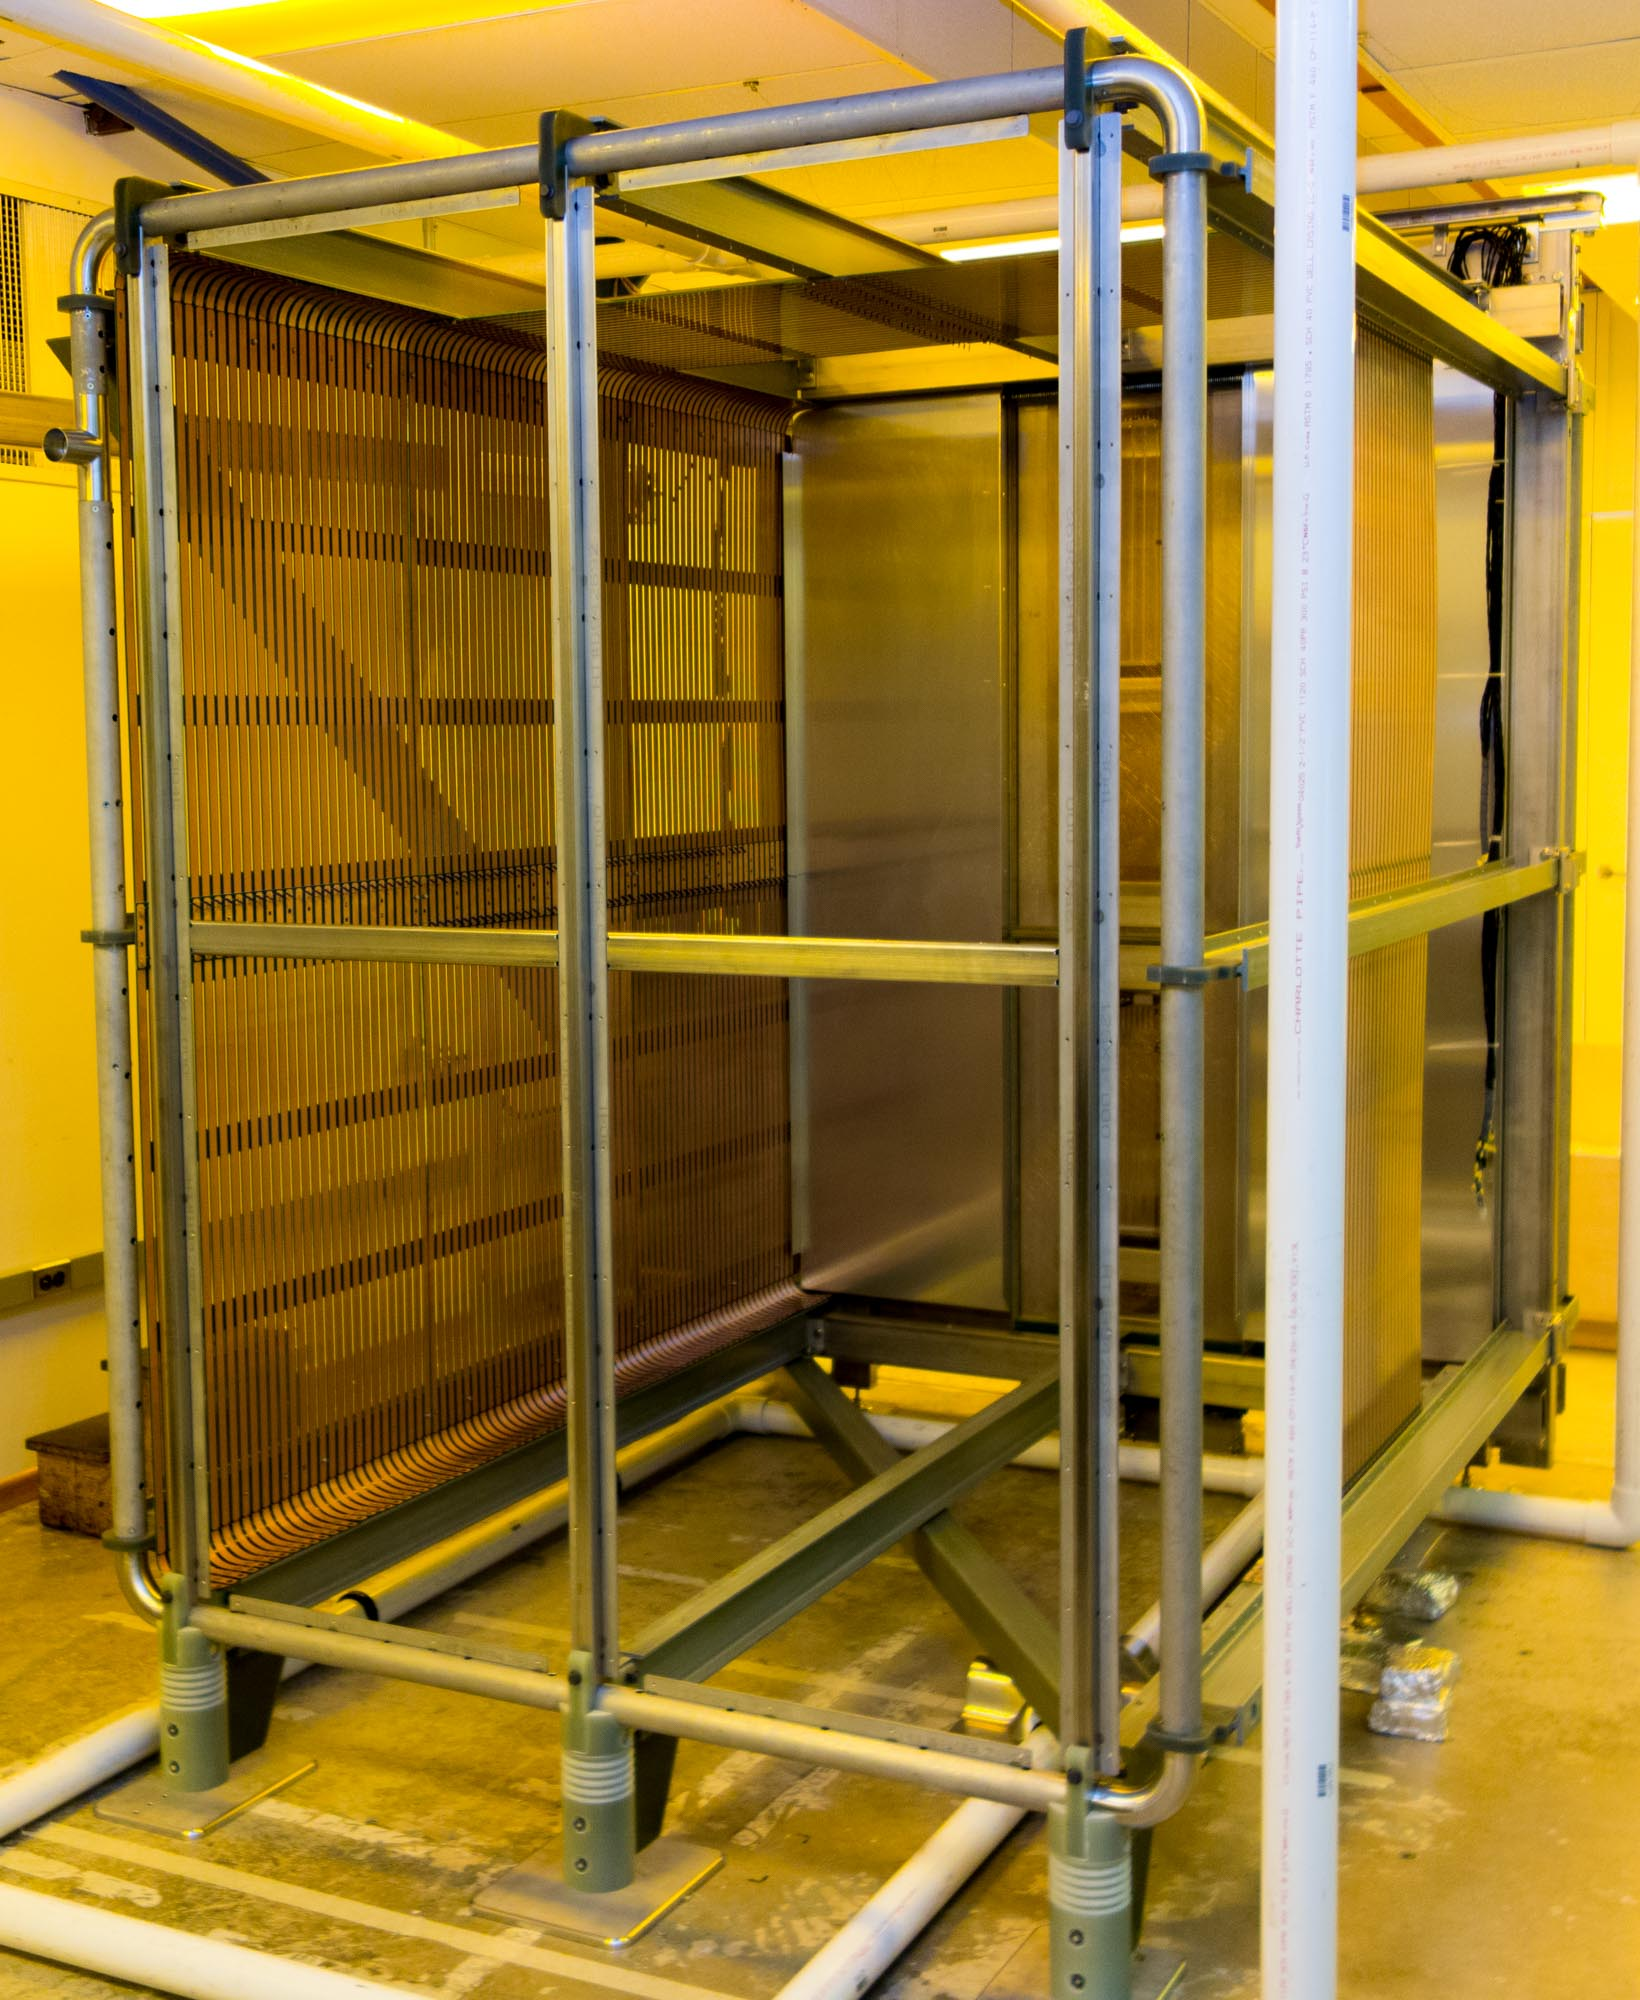
\includegraphics[width=0.35\textwidth]{35TTrial}  
\end{cdrfigure}

The Phase 2 prototype incorporates many of the design elements described in previous
sections of this document.
In many cases, these include novel features that have never previously been tested
in an operational TPC.
Rather than reiterate them all here, some of the more important
aspects are collected in Table~\ref{tab:35TDesign}.

\begin{cdrtable}[35t Design Elements]{lcl}{35TDesign}{35t Design Elements}
 Design Aspect& Section & How Tested\\ \toprowrule
Modular APAs with wrapped wires & \ref{subsec:v5-tpc-chamber-apa}&Build small-scale APA Modules with FD design\\
\colhline
Vertical Gaps between APAs &\ref{subsec:v5-tpc-chamber-apa}& Assemble APAs side-by-side.\\
&&Study reco'd tracks that cross the gaps.\\
\colhline
Horizontal Gaps between APAs &\ref{subsec:v5-tpc-chamber-apa}& Build two shorter APAs and stack vertically\\
&&Study reco'd tracks that cross the gaps\\
\colhline
APAs immersed in active volume &\ref{subsec:v5-tpc-chamber-apa}& Study reco'd tracks that cross APAs\\
\colhline
Cold Digital Electronics & \ref{subsec:fe_CMOS_digital} & Measure noise performance etc. {\it in situ}\\
\colhline
Waveguide-style Photon Detector& \ref{subsec:fe_CMOS_digital}&Install in APAs. Measure lightyield\\
\colhline
Triggerless-capable DAQ & \ref{sec:daq_intro} & Take data using multiple DAQ modes\\ 
\end{cdrtable}

\fixme{the xrefs in this table need to be fixed}

\subsection{Phase 2 Simulation, Reconstruction and Analysis}
As can be seen from Table~\ref{tab:35TDesign}, successful tests of many of the new 
design features requires simulation, reconstruction and analysis of 35t data. 
This will be done with the help of the LarSoft package, which is also used to simulate and 
reconstruct data from the ArgoNeuT and MicroBoone experiments.
Reuse of software developed for those experiments can greatly facilitate 35t development. 
However, the novel hardware features of the 35t prototype necessitate new software developments 
as well.  
Among the required new software developments are:
\begin{itemize}
\item{Code to break up the wrapped wires into as many as five individual linear segments. 
A hit on a single electronic channel can, in principle, be related to an induced signal on any of these segments.}
\item{``Disambiguation'' code to identify which of the possible wire segments was actually responsible
for the observed hit}
\item{Code for determining the start time of the event ($t_0$). Since the 35t prototype DAQ can
run ``triggerless,'' methods are needed for finding the $t_0$ in data. Information from the external 
scintillator paddles as well as the internal photon detectors can be used.}
\item{Code for ``stitching'' together track segments observed in different tracking volumes. 
Since hits can come from either side of the four APAs, there are effectively eight separate tracking volumes, 
which are treated as separate TPCs.}
\end{itemize}

With these simulation and reconstruction tools in hand, ``physics'' analysis of the data can be undertaken.
In addition to the analyses needed to validate the new detector design elements, there are also
some analyses of basic LArTPC performance that are needed as well.
Among the highest priority analysis tasks are:

\begin{itemize}
\item{Basic detector performance: signal/noise, purity measured with tracks, track direction resolution, 
photon detector light yield}
\item{Measurement of distortions due to space charge and field non-uniformity}
\item{Measurements of different types of particles: muons, protons, neutrons, pions}
\end{itemize}

The results obtained by operating the 35t Phase 2 prototype and the analysis of its data are expected
to be very valuable in defining the final far detector design. 
